\documentclass{beamer}


\usepackage[french]{babel}

\usepackage[T1]{fontenc}

\usepackage[utf8]{inputenc}


\usetheme{Warsaw}
\title{Nouvelle heuristique pour VRP}
\author{Clément Legrand}
\date{28 février 2018} 

\begin{document}

\section{Présentation heuristique}

\begin{frame}[plain]
\titlepage
\end{frame}

\begin{frame}
\underline{Intérêt}: heuristique simple à mettre en place, et performante.

Etapes de l'algorithme:
\begin{itemize}
\item Recherche solution initiale: Algorithme Clarke and Wright

\item Recherche de la "pire" arête

\item Optimisations locales ensuite par 3 opérateurs
\end{itemize}

\end{frame}

\section{Obtention de la pire arête}

\begin{frame}
Lien entre les solutions (presque) optimales ? 

Modèle prédictif qui distingue les solutions en s'aidant de caractéristiques:
\begin{itemize}
\item Largeur de la route
\item Profondeur de la route
\item Compacité de la route: moyenne des distances de chaque client au centre de gravité de la route.
\end{itemize}

	\centering
	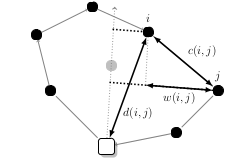
\includegraphics[height=0.4\textheight]{metrics.png}
	
\end{frame}

\begin{frame}
Description spatiale précise d'une arête avec ces caractéristiques. 
\begin{center}
$b(i,j) = \frac{[\lambda_w w(i,j) + \lambda_c c(i,j)] [\frac{d(i,j)}{max_{k,l}d(k,l)}] ^ {\frac{\lambda_d}{2}}}{1+p(i,j)}$
\end{center}

\begin{itemize}
\item $p$ représente le nombre de fois où l'arête a été pénalisée (initialement 0)

\item Les paramètres $\lambda_w$,$\lambda_c$ et $\lambda_d$ valent $0$ ou $1$, et sont choisis selon le type d'instance. 
\end{itemize}

\end{frame}

\section{Opérateurs locaux}

\subsection{Cross\_exchange}
\begin{frame}
Agit sur un couple de tournées, et essaie d'échanger toutes paires de séquence de clients consécutifs entre les deux routes. Complexité en $O(n^4)$: beaucoup trop...

\underline{Réduction}: si on connaît une arête à éliminer, on choisit la tournée correspondante. Et on ne s'intéresse qu'aux tournées qui ont des n\oe uds dans le voisinage de l'arête.

Complexité en théorie quadratique, mais proche de linéaire en général (beaucoup de solutions violent les contraintes)

	\centering
	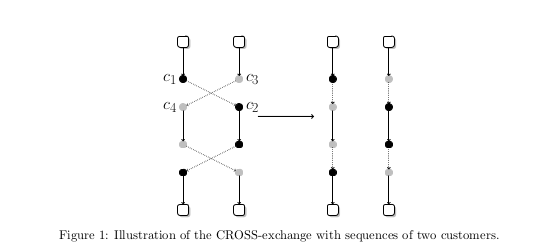
\includegraphics[height=0.4\textheight]{cross_exchange.png}
\end{frame}

\subsection{Ejection\_chain}
\begin{frame}
Agit (potentiellement) sur toutes les tournées. Commence par déplacer un client de la route $a$ vers la route $b$, de même en partant de $b$ vers $c$, jusque $l$ déplacements. 

	\centering
	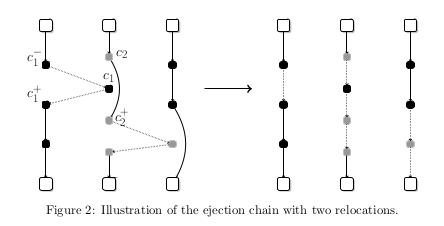
\includegraphics[height=0.4\textheight]{ejection_chain.png}
\end{frame}


\subsection{Lin-Kernighan Heuristic}
\begin{frame}
Utilisé en général sur TSP. Optimisation intra-tournée (chaque tournée est améliorée indépendamment ds autres). LK essaie de trouver un déplacement k-opt, pour améliorer la solution. Il commence par 2-opt, puis passe à 3-opt seulement si une meilleure solution a été trouvée. S'il atteint k, il exécute la meilleure i-opt et recommence à 2.

Complexité en $O(n^k)$. En général les changements sont mineurs et l'algo s'arrête après 2-opt.

\end{frame} 

\section{Améliorations}
\begin{frame}
Si on ne trouve plus d'améliorations
\begin{itemize}
\item Optimisation globale (application des opérateurs sur l'ensemble du graphe): très coûteux
\item Remise à zéro des pénalités
\item Changement de la fonction de pénalisation

\end{itemize}

\end{frame}

















\end{document}